\documentclass{beamer}

\usecolortheme[light]{solarized}

\beamertemplatenavigationsymbolsempty

\usepackage{graphicx}
\usepackage{hyperref}
\usepackage{booktabs}
\usepackage{amsmath}

\usepackage{tikz}
\usetikzlibrary{calc}

\title{Variability and queues}
\author{Vince \href{https://twitter.com/drvinceknight}{@drvinceknight}}
\date{}

\begin{document}

\begin{frame}
    \maketitle
	\begin{center}
		\includegraphics[width=.3\textwidth]{./img/CUident_CMYK.eps}
	\end{center}
\end{frame}

\begin{frame}
    \Large
	\begin{columns}
		\begin{column}{.5\textwidth}
			\begin{center}
				\begin{tabular}{cc}
					\toprule
					x &      y \\
					\midrule
					10.0 & 8.04 \\
					8.0 & 6.95 \\
					13.0 & 7.58 \\
					9.0 & 8.81 \\
					11.0 & 8.33 \\
					14.0 & 9.96 \\
					6.0 & 7.24 \\
					4.0 & 4.26 \\
					12.0 & 10.84 \\
					7.0 &  4.82 \\
					5.0 & 5.68 \\
					\bottomrule
				\end{tabular}
			\end{center}
		\end{column}
		\begin{column}{.5\textwidth}
            \pause
            \[
            \tilde x = 9.0
            \]
            \pause
            \[
            \tilde y = 7.5
            \]
        \end{column}
	\end{columns}
\end{frame}

\begin{frame}
    \Large
	\begin{columns}
		\begin{column}{.5\textwidth}
			\begin{center}
				\begin{tabular}{cc}
					\toprule
					x &      y \\
					\midrule
					10.0 & 9.14 \\
					 8.0 & 8.14 \\
					13.0 & 8.74 \\
					 9.0 & 8.77 \\
					11.0 & 9.26 \\
					14.0 & 8.10 \\
					 6.0 & 6.13 \\
					 4.0 & 3.10 \\
					12.0 & 9.13 \\
					 7.0 & 7.26 \\
					 5.0 & 4.74 \\
					\bottomrule
				\end{tabular}
			\end{center}
		\end{column}
		\begin{column}{.5\textwidth}
            \pause
            \[
            \tilde x = 9.0
            \]
            \pause
            \[
            \tilde y = 7.5
            \]
        \end{column}
	\end{columns}
\end{frame}

\begin{frame}
    \Large
	\begin{columns}
		\begin{column}{.5\textwidth}
			\begin{center}
				\begin{tabular}{cc}
					\toprule
					x &      y \\
					\midrule
					10.0 & 7.46 \\
					 8.0 & 6.77 \\
                    13.0 &12.74 \\
					 9.0 & 7.11 \\
					11.0 & 7.81 \\
					14.0 & 8.84 \\
					 6.0 & 6.08 \\
					 4.0 & 5.39 \\
					12.0 & 8.15 \\
					 7.0 & 6.42 \\
					 5.0 & 5.73 \\
					\bottomrule
				\end{tabular}
			\end{center}
		\end{column}
		\begin{column}{.5\textwidth}
            \pause
            \[
            \tilde x = 9.0
            \]
            \pause
            \[
            \tilde y = 7.5
            \]
        \end{column}
	\end{columns}
\end{frame}

\begin{frame}
    \Large
	\begin{columns}
		\begin{column}{.5\textwidth}
			\begin{center}
				\begin{tabular}{cc}
					\toprule
					x &      y \\
					\midrule
					 8.0 & 6.58 \\
					 8.0 & 5.76 \\
					 8.0 & 7.71 \\
					 8.0 & 8.84 \\
					 8.0 & 8.47 \\
					 8.0 & 7.04 \\
					 8.0 & 5.25 \\
					19.0 & 12.50 \\
					 8.0 & 5.56 \\
					 8.0 & 7.91 \\
					 8.0 & 6.89 \\
					\bottomrule
				\end{tabular}
			\end{center}
		\end{column}
		\begin{column}{.5\textwidth}
            \pause
            \[
            \tilde x = 9.0
            \]
            \pause
            \[
            \tilde y = 7.5
            \]
        \end{column}
	\end{columns}
\end{frame}

\begin{frame}
	\begin{center}
		\Large
		Are these sets of numbers the same?
	\end{center}
\end{frame}

\begin{frame}
	\begin{columns}
        \begin{column}{.5\textwidth}
            \begin{center}
                \includegraphics[width=.8\textwidth]{./img/anscombe-I.pdf}

                \includegraphics[width=.8\textwidth]{./img/anscombe-II.pdf}
            \end{center}
        \end{column}
        \begin{column}{.5\textwidth}
            \begin{center}
                \includegraphics[width=.8\textwidth]{./img/anscombe-III.pdf}

                \includegraphics[width=.8\textwidth]{./img/anscombe-IV.pdf}
            \end{center}
        \end{column}
    \end{columns}
\end{frame}

\begin{frame}
    \begin{center}
        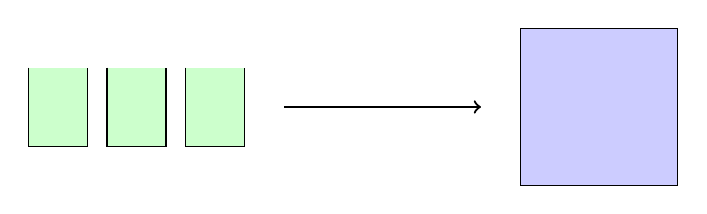
\begin{tikzpicture}
            % Arrow
            \draw [->, thick] (-3, 1) -- (-.5, 1);

            % Service center
            \draw [fill=blue!20] (0, 0) rectangle (2, 2);

            % Queue
            \draw [fill=green!20] (-4.25, 1.5) -- (-4.25, .5) -- (-3.5, .5) -- (-3.5, 1.5);
            \draw [fill=green!20] (-5.25, 1.5) -- (-5.25, .5) -- (-4.5, .5) -- (-4.5, 1.5);
            \draw [fill=green!20] (-6.25, 1.5) -- (-6.25, .5) -- (-5.5, .5) -- (-5.5, 1.5);
        \end{tikzpicture}
    \end{center}
\end{frame}

\begin{frame}
    \Large
    \begin{center}
        Mean time between arrivals: \(5.5\)\\
        Mean service rate: \(5.5\)\\
    \end{center}
\end{frame}

\begin{frame}
    \tiny
    \begin{center}
        \begin{tabular}{cccccc}
            \toprule
            ID       & Inter Arrival Time & Arrival Date & Service Time & Service Start Date & Service End Date\\
            \(n\)    & \(I_n\)            & \(A_n\)      & \(T_n\)      & \(S_n\)            & \(E_n\)\\
            \midrule
            1        &                    &              &              &                    & \\
            2        &                    &              &              &                    & \\
            3        &                    &              &              &                    & \\
            \dots    &                    &              &              &                    & \\
            \bottomrule
        \end{tabular}
    \end{center}
\end{frame}


\begin{frame}
    \begin{align*}
        I_n &= \text{random}  && \text{Inter arrival time}\\
        A_n &= I_{n-1} + I_n  && \text{Arrival date}\\
        T_n &= \text{random}  && \text{Service time}\\
        S_n &= \max(T_n, E_{n + 1}) && \text{Service start date}\\
        E_n &= S_n + T_n && \text{Service end date}\\
    \end{align*}
\end{frame}

\begin{frame}
    \Huge
    \begin{center}
        Demo.
    \end{center}
\end{frame}

\begin{frame}
    \begin{center}
        \begin{tikzpicture}[scale=2]
            \node (A) at (0,0) [draw] {RG};
            \node (B) at (2,0) [draw] {NH};
            \draw [->] (-1,0) -- (A);
            \draw [->] (3,0) -- (B);
            \draw [->] (-1,0) -- ($(A)+(-.5,0)$) -- ($(A)+(-.5,.5)$) -- ($(A)+(.5,.5)$) -- ($(A)+(.5,.1)$) -- ($(B)+(-.4,.1)$);
            \draw [->] (3,0) -- ($(B)+(.5,0)$) -- ($(B)+(.5,-.5)$) -- ($(B)+(-.5,-.5)$) -- ($(B)+(-.5,-.1)$) -- ($(A)+(.4,-.1)$);
            \draw [->] (3,0) -- (B);
            \node at ($(A) + (0,.8)$) {Divert?};
            \node at ($(B) + (0,-.8)$) {Divert?};
            \draw [->] (A) -- ($(A)+(0,-.5)$);
            \draw [->] (B) -- ($(B)+(0,.5)$);
        \end{tikzpicture}
    \end{center}
\end{frame}

\begin{frame}
    \Large
    \begin{center}
        \url{https://youtu.be/Z0lIzGA2ek8}
    \end{center}
\end{frame}

\end{document}
